% % Full page illustration
% \begin{figure}[!hbtp]
%     \centering
%     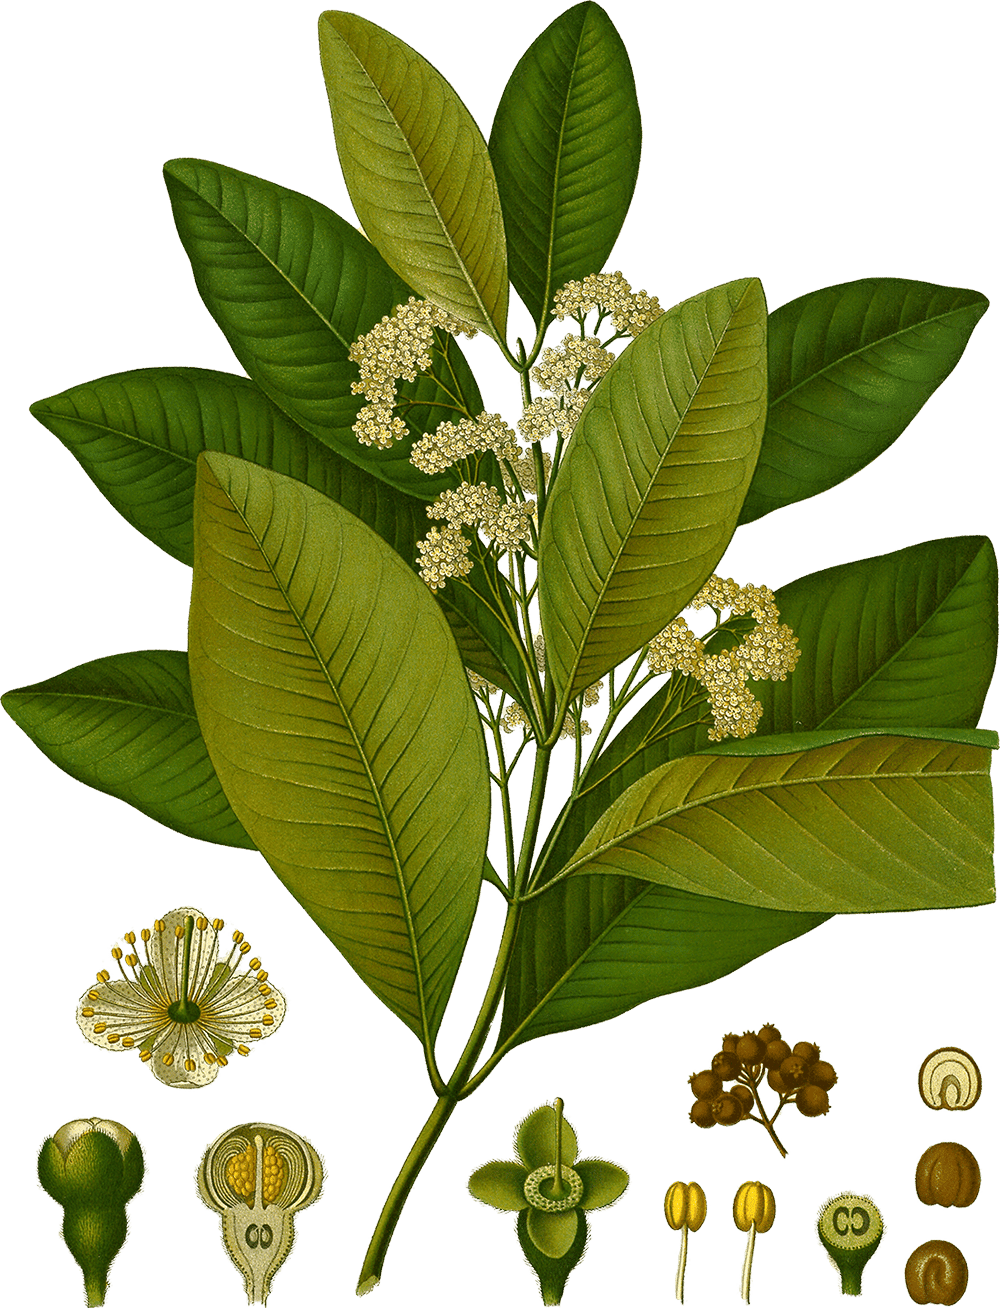
\includegraphics[width=\textwidth]{imgs/kohler/allspice_kohler_min.png}
%     \caption{\taxonn{Pimenta dioica}{(L.) Merr.} (syn. \taxonn{P. officinalis}{ Lindl.}), the allspice tree in Köhler's Medicinal Plants \pvolcite[]{2}[174]{kohler_kohlers_1887}.}
%     \label{fig:kohler_allspice}
% \end{figure}


% \begin{wrapfigure}{O}{0.5\textwidth}
%   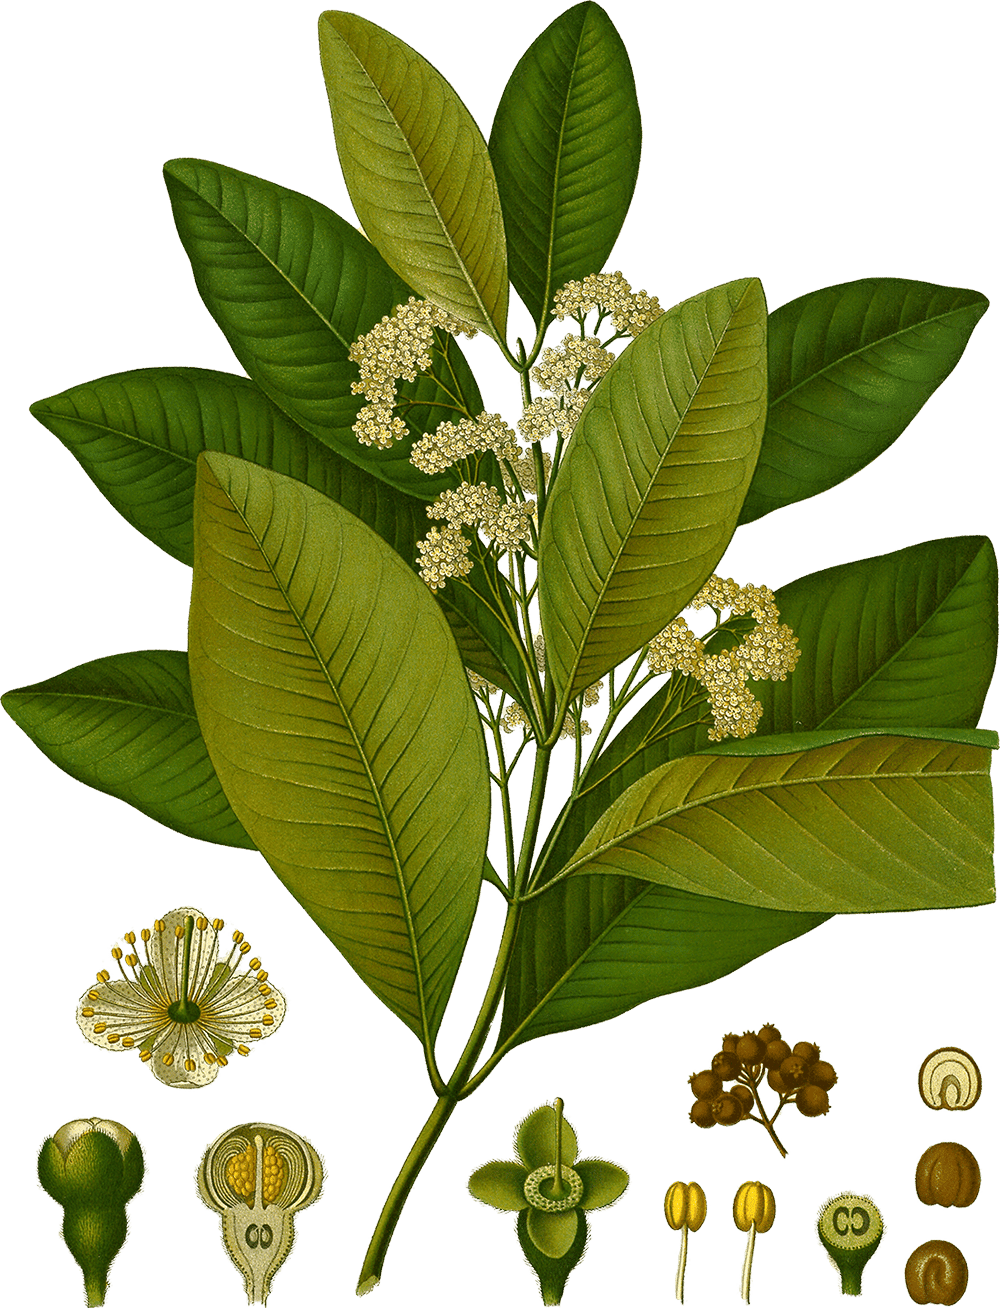
\includegraphics[width=0.5\textwidth]{imgs/kohler/allspice_kohler_min.png}
%   \caption{\textit{Pimenta dioica} {\small(L.) Merr.} syn. \textit{P. officinalis} {\small Lindl.} the allspice tree in Köhler's Medicinal Plants \pvolcite[]{2}[174]{kohler_kohlers_1887}.}
% \end{wrapfigure}


% \begin{wrapfigure}{o}{0.5\textwidth}
%     \includegraphics[width=0.5\textwidth]{imgs/spices/allspice.jpg}
%   \caption{Allspice berries}
% \end{wrapfigure}

\section{Allspice}
\label{sec:allspice}

\begin{spice}\label{spice:allspice}
\textsc{Allspice} \hfill \href{https://powo.science.kew.org/taxon/196799-2}{POWO} \\
\textbf{English:} \textit{allspice}; \textit{pimento; Jamaica pepper}. 
\textbf{Arabic:} {\arabicfont{فلفل إفرنجي}} \textit{fulful ifranjī} [Frankish pepper]. 
\textbf{Chinese:} {\tc{多香果}} \textit{duōxiāngguǒ} [many-spice-fruit]. 
\textbf{Hungarian:} \textit{szegfűbors} [clove-pepper]; \textit{jamaicaibors} [Jamaican-pepper]; \textit{amomummag} [amomum-seed].  \\
\noindent{\color{black}\rule[0.5ex]{\linewidth}{.5pt}}
\begin{tabular}{@{}p{0.25\linewidth}@{}p{0.75\linewidth}@{}}
Plant species: & \taxonn{Pimenta dioica}{(L.) Merr.} (syn. \taxonn{Pimenta officinalis}{Lindl.}) \\
Family: & \textit{Myrtaceae} \\
part used: & unripe fruit; leaf \\
Region of origin: & S. Mexico to C. America; Caribbean \\
Cultivated in: & Jamaica; Mexico; Honduras \\
Color: & dark brown \\
\end{tabular}
\end{spice}

\begin{figure}[!ht]
	\vspace{-4ex}
	\centering
	\subfloat[\centering berries]{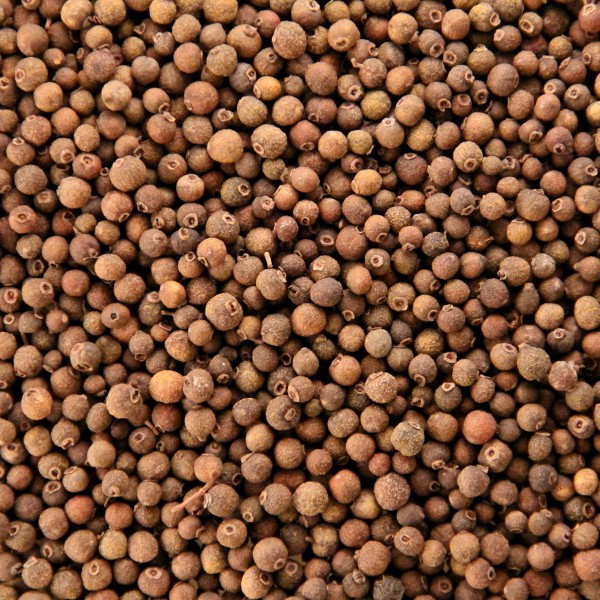
\includegraphics[width=0.3\linewidth]{imgs/spices/allspice-1.jpg}}
	\hfill
	\subfloat[\centering powder]{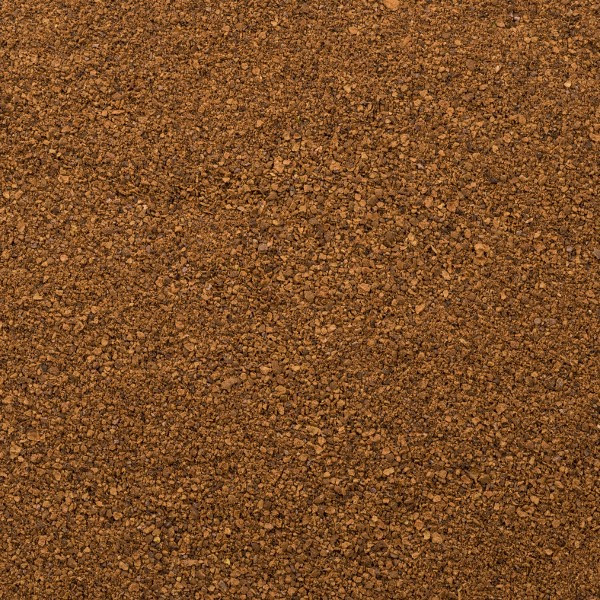
\includegraphics[width=0.3\linewidth]{imgs/spices/allspice-2.jpg}}
	\hfill
	\subfloat[\centering leaves]{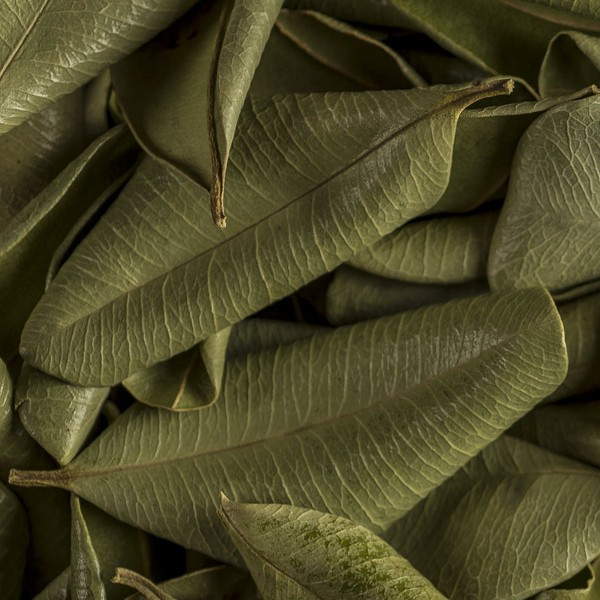
\includegraphics[width=0.3\linewidth]{imgs/spices/allspice-3.jpg}}
	\caption{Allspice berries, powder, and leaves from \taxon{Pimenta dioica}.}
	\label{fig:allspice_imgs}
\end{figure}

\begin{note}
	Introducing the \textit{Spice profile box}. As it can be seen above in \textit{Spice profile} \ref{spice:allspice} presenting allspice, this business-card-like environment gives a quick reference of the spice under scrutiny in a concise way. This is intended to be a convenience for the reader to return and glance back at brief, factual information about a particular item whenever necessary. The box also contains a clickable link to the related plant species in a botanical database, \gls{POWO}, where more information can be found, such as the plants' biodiversity, distribution, botanical synonyms, as well as images of specimens.
\end{note}

%DESCRIPTION
Allspice, also known as pimento and Jamaica pepper, refers to the dried unripe fruits of a tropical evergreen tree growing in the Caribbean: the \taxon{Pimenta dioica}. The dried berries are dark brown, hard to the touch, and 4--6 mm in diameter (thus larger than black pepper). Their signature crown is by a small ring of the calyx \autocite[210]{van_wyk_culinary_2014}. It is one of the few spices that do not come from the East; chili, vanilla, and allspice are the traditional three when one is listing spice products native to the Americas (disregarding cacao which is not considered a spice today). It is also the only spice that is exclusively cultivated on the western hemisphere \autocite[21]{duke_crc_2002}. The term \textit{allspice} is a coinage playing on the notion that the flavors and aroma of allspice is similar to that of clove, cinnamon, nutmeg, and black pepper \autocite[717]{mabberley_mabberleys_2017}---the most popular spices in Europe at the time when Europeans got in contact with this New World spice. People who only saw ground allspice but not whole, often tend to think that is in fact a spice mixture, after its name and rich flavor profile. Usually ground to powder, allspice is one of the key ingredients of Caribbean cuisine, especially jerk style dry-rub meat preparation. It is also used in European sausage making, pickling, baking, and flavoring liqueurs, it an overall ``handy spice''.\footnote{The Icelandic name is \textit{allrahanda}, literally `of all hands', meaning `for various purposes'; showing its multifaceted uses.} It also found its way into some Middle Eastern spice blends.


\begin{note}
\label{note:pimento}
Allspice is sometimes called pimento, which is also the name of a cultivar of \taxon{Capsicum annuum}, famous from the Southern United States appetizer pimento-cheese. It is therefore important not to confuse allspice with the heart-shaped mild cherry peppers that North Americans also call pimiento or pimento. 
\end{note}

\subsection{The Botany, Origin, and  Cultivation of Allspice}

%PLANT
The allspice tree is a small mid-canopy tree or shrub with smooth, bay-like leaves and tiny white flowers. The berries turn dark purple if left to ripe, and the leaves and the bark are also aromatic \autocite[279]{riffle_tropical_1998}. Belonging to the myrtle family (\textit{Myrtaceae}), allspice is related to other aromatic trees, such as clove, eucalyptus, and the bay rum tree. Its binomial name is made up of \textit{pimenta}, the Portuguese (or corrupted Spanish) equivalent of `pepper', and \textit{dioica} `of two houses' (Greek \textit{di-} from \textit{dyo} `two' and \textit{oikos} `house'), indicating that the male and female flowers are found on different plants \pvolcite[]{2}[166]{peter_handbook_2012}.

%ORIGIN
Allspice is indigenous to the regions ranging from Southern Mexico to Central America and the Greater Antilles of the Caribbean, especially Jamaica \autocite[146]{czarra_spices_2009}. Where naturalized, it spreads by birds carrying the seeds. Allspice has been since introduced to a few neighboring places, such as Colombia, Venezuela, and Florida \autocite[][146]{powo_pimenta_2022}. In 1885 it was introduced from Jamaica to Hawaii and Kauai, 
% where it is designated as one of the most invasive horticultural plants of Hawaii \autocite{gisd_pimenta_2022}, 
and it even reached Tonga.

%CULTIVATION
Allspice is cultivated as a crop in a few countries, notably in Jamaica, Mexico, and to a lesser extent in Honduras and Grenada. The primary producer and the source of the highest quality being Jamaica. Saplings are grown from seeds, then soon transplanted when still small. The trees need well-drained soil and humid conditions \autocite[210]{van_wyk_culinary_2014}. It is one of the only spices that no one managed to grow in the East, transplantation efforts were quickly abandoned, and its commercial cultivation is confined to the Americas \autocite[21]{duke_crc_2002}. 
%HARVEST
Harvesting happens similarly to how black pepper is harvested; the still green, unripe fruits are picked by hand, and then dried under the sun.

%CHEMISTRY
The flavor of allspice mainly comes from the component eugenol, which is dominant both in the fruit and the leaves, but other compounds also add to the complexity of its aroma. Eugenol---also called clove oil, for it constitutes 80-90\% of the essential oil from clove buds \autocite[166]{barnes_herbal_2007}---is widely used as a flavoring agent by the food industry and in pharmacology, and is also found in cinnamon, nutmeg, and bay leaves. It has antiseptic, antibacterial, anesthetic, and analgesic properties \autocite{ulanowska_biological_2021}. The leaves of a related plant called the West Indian Bay Tree (\taxon{Pimenta racemosa}) is used to produce bay rum, a popular essential oil used by the perfume industry for its spicy notes. 
% \todo{Contrary to popular belief, none of the above seems to be an ingredient in Old Spice\footnote{\url{https://www.fragrantica.com/perfume/Shulton-Company/Old-Spice-Original-14746.html}}}


% %USES
% \subsection{Culinary and Medicinal Uses}


% green 2006

% www.foodreference.com/html/fallspice.html
% The fruit and leaf oil are also used in men's toiletries - any time you see the word 'spice' in the name, such as in 'Old Spice' you can be sure that the fragrance comes at least in part from allspice oil. ??? no proof
% Pimento (Allspice) wood is used in Jamaica to cooked 'jerked' meats.

% Wyk:
% Allspice has become popular in some Western and East European countries, initially as a spice to replace cardamom. It is used to flavor a wide range of dishes, including meat stews, sausages, salted beef, pork, meat pastries, pickles, sauces and stuffings. Allspice is an essential ingredient of Caribbean cuisine (e.g. jerk seasoning). It is used in Scandinavian smorgasbord, as well as fish, cheese and vegetable dishes. Mexicans use it in moles. Allspice is popular in Great Britain, where it is used in stews, sauces, confectionery, puddings and the traditional Christmas cake. Jamaican pimento dram and French liqueurs such as Benedictine and chartreuse are flavored with allspice.2 The spice, fruit oil or oleoresin extracts are commonly used in food processing, especially to flavor charcuterie items such as sausages, ham, salami and canned meats, as well as curry powders, condiments, relishes, ketchup, pickling spices and gravy mixtures. Leaf oil is used in ice creams, puddings, confectionery and liqueurs. 

% Czarra 146:
% Allspice is primarily used in the food industry in pickles, sausages, ketchup and canning meat. It can be also used as a spiced tea mix, in soups and curries and as a pickling spice.

% The fresh leaves of the allspice tree are used similarly to bay leaves in cooking, but they cannot be stored dry as opposed to the bay leaf; they lose their aroma.

%Where the tree is native, the wood is used to smoke meat.

% Duke 245
% Other Uses (Allspice) — Allspice of commerce is the dried unripe fruit, used as a condiment; in baked goods, chutney, ice cream, ketchup, mixed spices, pickles, sauces, soups; and in flavoring sausages and curing meats. Allspice powder consists of whole ground dried fruit. It’s called “allspice” because it supposedly embraces the aromas of cinnamon, cloves, and nutmeg. To make an allspice substitute, merely combine one part nutmeg, two parts cinnamon, and two parts clove (RIN). Mexican Indians used allspice to flavor chocolate. I use it to flavor eggnog. Allspice is an essential ingredient of the rubs and marinades used in seasoning Jamaican jerked foods, which are also flavored by the smoke of pimento wood fires (FAC). In Jamaica, a local drink called “pimento dram” is made of ripe fruits and rum. It is regarded as a panacea. Allspice is used in such liqueurs as Benedictine and Chartreuse. A volatile oil, extracted from the spice and leaves, is used to flavor essences and perfumes and as a source of eugenol and vanillin. The oil is also used in flavoring beverages, candies, chewing gums, liqueurs, meats and sauces, and in Asian perfumery and shaving lotions. Bahamians make a pleasing tea from the leaves. Costa Ricans use the leaves as a spice. Many ethnic groups use the leaves in tea. Saplings are used as walking sticks and umbrella handles (DAD, FAD).

% Wiki:
% Allspice is also one of the mainly used spices in Polish cuisine (used in most dishes, soups and stews) and is commonly known under the name English herb (Polish: ziele angielskie). 
% At the time allspice was encountered by Christopher Columbus during his second voyage to the New World, it was found only on the island of Jamaica, where the plant was readily spread by birds. Allspice was introduced into European and Mediterranean cuisines in the 16th century. To protect the pimenta trade, Jamaican growers guarded against export of the plant. Many attempts at growing the pimenta from seeds were reported, but all failed. Eventually, passage through the avian digestive tract, whether due to the acidity or the elevated temperature, was found to be essential for germinating the seeds,[7] and successful germination elsewhere was enabled. Today, pimenta grows in Tonga and Hawaii, where it has become naturalized on Kauaʻi and Maui.[8] It continued to be grown primarily in Jamaica, though a few other Central American countries produced allspice in comparatively small quantities.[9]

% Duke 21?

% the allspice fruits were used to preserve meats on long voyages. These preservative activities are due to some of the aromatic and antiseptic compounds which abound in allspice (anethole, caryophyllene, eugenol, linalool, pinene, and terpinene).

\subsection{The History of Allspice}

% https://journals.openedition.org/ethnoecologie/6261

There is not much we know about allspice before the arrival of the Europeans, except that the Aztecs used it to spice up their chocolate drink \autocites[27]{farrell_spices_1985}, although \textcite[145, 177]{dalby_dangerous_2000} doubts this was the case that early on. According to \textcite[21]{duke_crc_2002}, the Maya used allspice for embalming. We know that it reached Europe as a consequence of Christopher Columbus's voyages. Spanish colonizers must have encountered allspice in the West Indies sometime after Columbus and his crew explored the islands of Hispaniola, Cuba, and Jamaica, and the year 1494 is reported \autocite[12]{opara_culinary_2021}. Columbus himself did not find it. In fact, he did not recognize any spice he was so keen on finding---pepper, cloves, nutmeg, cinnamon---but kept himself and his patrons in the delusion that he will. In his first letter to Ferdinand and Isabella he writes: ``On this island there are many spices and great mines of gold and other metals. [...] I believe that I have found rhubarb and cinnamon.'' \autocite[10-18]{columbus_spanish_1893} ---in reality, he had none.\footnote{Columbus's first letter of his first voyage, sent on March 4, 1493 from Lisbon to the Spanish court (and its translation) is also available online at King's College London. Transcription: \url{http://www.ems.kcl.ac.uk/content/etext/e021.html}, translation: \url{http://www.ems.kcl.ac.uk/content/etext/e022.html}}

He was adamant that the islands he \textit{discovered} were full of spices and brought up excuse after excuse (out of season, etc.) after every voyage he returned with no spice \autocite[149]{dalby_dangerous_2000}. He also believed that he was in India or Cathay, on one of the outlying islands. Between apologies, Columbus also promised more gold, silver, cotton, mastic, and slaves. As \textcite[150]{dalby_dangerous_2000} reports, what he recorded in his private journal is a bit more honest and realistic version of events: ``I think that many trees and plants grow here which will be highly valued in Spain for dyes and medicinal spices. But I am sorry to say that I do not recognize them.'' Columbus repeatedly regrets his ignorance in botany in his journal \autocite[see also][57]{columbus_journal_2010}.

Interestingly, authors love to claim that Columbus brought back allspice (together with vanilla and chili): ``He returned with allspice from the West Indies, chilies from Mexico and vanilla from Central America.'' \autocite[17]{craze_spice_1997}, and ``Columbus brought it back to Europe thinking it was pepper.'' \autocite[146]{czarra_spices_2009}, or ``Though he did not find the Spice Islands, Columbus brought allspice, vanilla and red peppers from the West Indies back to his Spanish supporters.'' \autocite[1]{parthasarathy_chemistry_2008}. This is not true, he most likely never even saw allspice, but it was reported him that it is there and can be cultivated, along with cinnamon, and mulberry for silk production \autocites[151]{colon_life_1959}. Columbus returned from his first voyage of 1492--93 with some gold nuggets and jewelry, pearls, a hammock, tobacco, the turkey, and a few poor captured Taínos, but no spices were presented to the Spanish monarchs Ferdinand and Isabella. He did bring back pineapple and cassava \autocite[11]{turner_spice_2004}. 

Diego Álvarez Chanca, the court appointed physician who accompanied Columbus on his second expedition in 1493 is often credited with bringing home both chili, and allspice \autocites[]{mccormick_history_nodate}, but in his 1494 letter describing the flora and fauna, he only mentions \textit{agi}, also \textit{axi}---modern Spanish \textit{ají} from Taíno---\autocite[see][34]{corominas_breve_1987}, and that the natives use it to season their food, with what we now know as \taxon{Capsicum annuum}: the chili pepper \autocite[311]{chanca_american_2003}.

In the following century the Spanish tried to turn Mexico into a spice plantation by transplanting eastern spices, an effort that mostly failed. Only after this did the colonizers start to pay proper attention to native spices \autocite[6]{machuca_past_2020}. 

Francisco Hernández de Toledo, King Philip II's court physician and naturalist spent 7 years in New Spain between 1571--1577, studying its species and conducting interviews with the natives. He was the first to formally describe allspice. He called it \textit{Pipere Tavasci} `Tabasco pepper' (today \textit{Pimienta de Tabasco}, after the region of Tabasco, famous today for a brand of hot sauce. Hernández also recorded the Nahuatl name of allspice: \textit{xocoxochitl} `sour flower'.\footcite[cf.][xococ; xochitl]{ond} Hernández likens the flowers to pomegranates, and and the aroma to that of orange blossoms, describing it to be very pleasant and attractive, with a sharp taste of the fruit. \autocite[2]{hernandez_cuatro_1615}. In \textcite{machuca_past_2020}'s translation:

\begin{quote}
    ``Xocoxochitl meaning sour flower, is a large tree, with leaves like those of the oranges, red flowers like a pomegranate, but with an aroma like the orange blossom, and in such a smooth and pleasant way, that even the leaves of the tree add to its attraction: the fruit is round, and hangs in clusters, which at first appear green, and then beige, and finally towards black: it is sharp and scathing to taste, and good-smelling'' 
\end{quote}

According to \textcite{machuca_past_2020}, although allspice was known by the Spanish from early on ``there are few historical records of its production and trade'', and only in the \nth{18} century started they to consider American products to have economic potential.
 
Allspice berries are around 30\% larger then peppercorns, and since their color and shape resembles black pepper, and it gave a spicy taste to food, it is no wonder that the Spanish called them \textit{pimiento} `pepper'. The Portuguese version is \textit{pimento}, and later the botanical name \textit{Pimenta} was given to the genus of plants related to allspice \autocite[26]{farrell_spices_1985}. I disagree with the often repeated trope that the Spanish explorers mistook allspice berries for pepper and called them \textit{pimiento} ``by mistake''\footcite[allspice \link{https://www.britannica.com/plant/allspice}]{britannica_allspice_nodate}, these people knew exactly what they were looking for, and that what they have found is not the mighty black pepper; but for them it was a kind of pepper. The crew showed samples of pepper and cinnamon to presumably confused Native Americans hoping for directions, and as Columbus wrote in his journal on the \nth{4} of November, 1492, they indicated by sign language that there is a lot of it around \autocites[21]{duke_crc_2002}[67]{columbus_journal_2010}. The Europeans, however, soon recognized the value of allspice, even if it was not the expensive black pepper, but still more pungent and exotic than some cheap Old World substitutes, the juniper and myrtle berries (which are very similar to allspice in appearance and usage)  \autocite[150]{dalby_dangerous_2000}.

In short, allspice was introduced to Europe by the Spaniards in the \nth{16} century, its import was first recorded in 1601, according to \textcite{britannica_allspice_nodate} and \textcite[26]{farrell_spices_1985}. After 1655, when Jamaica became a British colony for nearly three centuries, the Brits developed a taste for allspice and started to use it to season meat dishes, sauces, and pickles \autocite[74]{green_field_2006}. They were also responsible for its spread to some extent which is illustrated by the names of allspice in some languages, e.g. Polish \textit{ziele angielskie} `English herb'.

% Allspice was first exported to Europe in 1601 as a substitute for cardamom. ?? Farrell 26

% https://www.mexconnect.com/articles/3799-fragrant-flavorful-allspice-an-essential-mexican-seasoning/

% peter 2 167
% The berries reached London in 1601 as described by Clusius in his Liber Exoticorum and the plants were first cultivated in England in a hot house in 1732 (Weiss, 2002). Before World War II, allspice was more widely used than today; however, during the war many trees were cut down and there was a shortage of the spice. Although cultivation was taken up after the war, production never fully recovered.


\subsection{The Names of Allspice}

Allspice is a fascinating case, because it gives us examples for a plethora of names that showcase us many of the motivations, mechanisms, and solutions people choose when naming spices. As I mentioned before, some people are puzzled if allspice is a spice blend or not. The names in some languages often just add to the confusion, for example French \textit{quatre-épices} (lit. `four spices') can have the sense `allspice', but also `a kind of spice mix' made up of four different spices.\footcite[quatre-épices \link{https://www.cnrtl.fr/definition/quatre-\%C3\%A9pices}]{tlfi}


% All these names can be explained by the characteristics, use, and journey of allspice. Let us now consider the names in English, Arabic, and Chinese.

\subsubsection{English}

\begin{etymology}\label{ety:allspice}
\textbf{English} \textit{allspice}, from \textit{all} + \textit{spice}; after the flavor profile that resembles the combined aroma of cloves, nutmeg, cinnamon, and black pepper, 1621\footnote{\textcite[s.v. allspice]{oed}}
\end{etymology}

\begin{note}
	Introducing the \textit{Etymology box}. This environment, as seen above in \textit{Etymology} \ref{ety:allspice}, offers a quick look at a words' origins and development.
\end{note}

Since its introduction to the spice cabinet, allspice has been known by many names from which currently \textit{allspice} \index{allspice|textbf} seems to be prevailing. \textit{Allspice} was formed by compounding \textit{all} and \textit{spice}, for its flavor was perceived to be a combination of four characteristic spices that the Europeans knew and sought after: black pepper, cinnamon, cloves, and nutmeg.\footcites[allspice]{oed}[]{britannica_allspice_nodate} It was first recorded in 1621: ``Ambergreese, nutmegs, and all spice.''\footcite[allspice]{oed}, and probably inspired the French \textit{toute-épice} `all-spice', attested in 1762.\footcite[toute-épice \link{https://www.cnrtl.fr/etymologie/toute-\%C3\%A9pice}]{tlfi}

Sadly, the original word for allspice was lost with the demise of the native Taíno people of the Caribbean, nevertheless we got Taíno\footnote{Taíno is a now extinct Arawakan language.} words such as barbecue, \textit{cassava}, \textit{guava}, \textit{hammock}, and \textit{tobacco} \autocite[229]{rafinesque_american_1836}. As we concluded before, it is assumed that it was the Spanish who first got in contact with the allspice berry, and that they simply called it \textit{pimienta} `pepper'.

\begin{etymology}\label{ety:pimento}
\textbf{English} \textit{pimento} `allspice; sweet pepper', ca. 1660
< partly \textbf{Portuguese} \textit{pimenta} `allspice; sweet pepper; black pepper'
< and partly \textbf{Spanish} \textit{pimiento} `hot and sweet pepper; formerly also black pepper; pepper plant of both kinds', earlier \textit{pimienta} `black pepper; peppercorn; ground pepper' \nth{13} c., 1495
< \textbf{Medieval Latin} \textit{pigmenta} `plant juice; food seasoning; condiment; spices; perfumes', plural of \textit{pigmentum}
< \textbf{Latin} \textit{pigmentum} `colour, paint; ointment; drug; spiced wine', from \textit{pingō} `to paint' + \textit{-mentum} `instrument'\footnote{\textcite[s.v. pimento]{oed}; \textcite[s.v. pimento]{oed}; \textcite[s.v. pimiento]{oed}; \textcites[415]{gomez_de_silva_elseviers_1985}[495]{corominas_breve_1987}; \textcite[s.v. pigmentum]{lewis_latin_1879}}
\end{etymology}

For a long time \textit{pimento} (and to a much lesser extent \textit{pimiento})---the words for `pepper' in Portuguese and Spanish, respectively---was commonly used in English to refer to allspice. This is still the case in Jamaican English for example, where the term \textit{allspice} is not used. In North American English however, \textit{pimento} now rather refers to a small, round variety of chili pepper (\taxon{Capsicum annuum}), commonly known as cherry pepper explained in \cref{note:pimento}. 

The corruption and mix-up between the English words \textit{pimento} and \textit{pimiento} and their origins is as confusing as it gets. For the sake of a clear understanding, let us first consider the modern names for allspice in Spanish: \textit{pimienta de Jamaica}, and Portuguese: \textit{pimenta-da-jamaica}. In both cases, \textit{pim\-(i)enta}, with a final \textit{-a}, means `pepper', referring to peppercorns of the usual black and white pepper (\taxon{Piper nigrum}). In Spanish and Portuguese, the words endings of \textit{-o} and \textit{-a} mark the grammatical gender, the significance of which dissipates in English. It is important to remember however, that the Spanish form \textit{pimienta} emerged first from a Latin neuter plural suffix in the \nth{13} century. Thus, perhaps a century or so later when the word \textit{pimienta} was already embedded in Spanish, speakers perceived the word as a feminine noun, and a vacuum of a masculine counterpart emerged. This allowed for a practical differentiation by gender between the peppers of the Old Word and the New World. \textcite[459]{corominas_breve_1987} explains that \textit{pimiento} derived from \textit{pimienta}, and it was first applied in the Americas for the red fruits of the chili.

\textcite[415]{gomez_de_silva_elseviers_1985} makes the most compact distinction: ``\textit{pimienta} `(black) pepper; allspice', \textit{pimiento} `(hot and sweet) pepper' ''. In contemporary Spanish, \textit{pimiento} (the masculine form) refers to the fruits and plants of the \textit{Capsicum} family, e.g. the numerous spicy chilies and mild bell peppers of red, green, and yellow, while \textit{pimienta} (the feminine form) refers to the small round fruits of black and white pepper and its powdered forms. The distinction seems consistent, belonging to this latter group see for example \textit{pimienta dulce} `sweet pepper', and \textit{pimienta gorda} `fat pepper' both of which refers to allspice, not to be confused with \textit{pimiento dulce}, which refers to sweet paprika powder.\footcite[pimiento, -a]{dle}

\textit{Pimento} in English is a partly Portuguese, partly Spanish borrowing, while \textit{pimiento} comes from Spanish. In fact, it is explained in the \gls{OED} that in the `allspice' sense of the word, \textit{pimento}, from Portuguese \textit{pimenta (da Jamaica)}, went through an alteration influenced by the Spanish word form, which is not attested in the `allspice' sense. Ergo, Spanish \textit{pimiento} maybe did not refer to allspice in Spanish at the time when the borrowing happened. And if so, \textit{pimento} is a borrowing from Portuguese \textit{pimenta} meaning `pepper' and, as \textit{pimenta da Jamaica}, `allspice', influenced by Spanish \textit{pimiento} `chili, sweet pepper', also in the sense of the pepper plants of both kinds (chili and black). Spanish \textit{pimiento} formerly had the sense of `black pepper, peppercorns, and ground pepper' (before 1495), with an earlier form \textit{pimienta} (\nth{13} century), now usually in sense ground pepper and peppercorns\footcite[pimento]{oed}. The Portuguese connection is only discussed by the \gls{OED}, other dictionaries do not mention it. A direct Spanish borrowing is also plausible if we consider that it was the Spanish who most likely brought it back first, they probably called it \textit{pimiento/-a}, and they were responsible for its subsequent diffusion in Europe. English spellings varied greatly of this this Romance word, using forms such as \textit{piemente} in the late 1600s. 

The origin of these words is the classical Latin \textit{pigmentum} `a material for coloring, a color, paint, pigment', with a transferred meaning `the juice of plants' in post-classical Latin.\footcite[pigmentum \link{http://www.perseus.tufts.edu/hopper/morph?l=pigmentum\&la=la\&can=pigmentum0\#lexicon}]{lewis_latin_1879} The word \textit{pigmentum} is made up of \textit{pingō} `to paint' and \textit{-mentum}, a suffix denoting an `instrument, medium', well recognizable from Romance languages and English (i.e. excite\textit{ment}).
According to \textcite[459]{corominas_breve_1987}, Catalan \textit{pimienta} is attested in the \nth{13} century and it comes from the plural (\textit{pigmenta}) of Latin \textit{pigmentum} `coloring, paint', which already meant `drug, ingredient', and later, `condiment' in Medieval Latin. Derived from this, in 1495 \textit{pimiento} was applied to the the plants bearing the pungent red fruits of the Americas. \textit{Pigmentum} also entered English as \textit{pigment} `paint, dye, ingredient in an ointment, drug'. According to the \gls{OED}, Medieval Latin \textit{pigmentum} also referred to spiced drinks (\nth{9} century), perfumes, and hence spice in general. Old French cognates support this, \textit{pigment} had the sense of `balm, fragrant spice' in the \nth{12} century, Anglo-Norman \textit{pigment/piment} meant `spice, spice wine'\footcite[pigment]{oed}, and Middle English \textit{pihmentum} (\nth{12} century, later \textit{piment}) had a sense of ``a spiced drink, a remedy or concoction containing spices'',\footcite[pigment]{oe} ``a sweetened, spiced wine used for refreshment and in medical recipes; a medicinal potion''.\footcite[piment]{med} \textit{Piment} in French were later applied for chili, especially the cultivar of cayenne pepper. (The \gls{OED} points to the sense `cayenne pepper' in a ``\nth{10} century French source'', which must be an error.)


Allspice is also known as \textit{Jamaica pepper}, for it mainly grows on the island and the historical reasons described above. Many languages calqued \textit{pimienta de Jamaica} from Spanish, or another transmitting language (e.g. Italian \textit{pepe della Giamaica}). \textit{Jamaica pepper} was first recorded in 1661: ``A kind of Pepper, that tastes like Cloves, and very Aromatick (known by the name of Iamaica-Pepper)''.\footcite[Jamaica]{oed}

The name \textit{myrtle pepper} \index{pepper!myrtle} echoes the similarities of the allspice tree with European myrtle (\taxon{Myrtus communis}), especially after the resemblance of their purple berries. Beyond the physical resemblance, myrtle berries are also edible, and are also dried to add to pepper mills as a spice. Furthermore, the European myrtle has aromatic leaves and wood as well, and it is used to grill and smoke meat in Southern Europe since Roman times, especially on Sardinia and Corsica; the same way the Caribbean people use allspice wood and leaves. The myrtle berry appears in Roman and Greek mythology as well \autocite[186]{van_wyk_culinary_2014}.

The name \textit{clove pepper} has ``chemical reasons'', namely that this name arises from the aroma of allspice that reminded people of clove. This is due to its eugenol content we discussed above. \textit{Szegfűbors} lit. `clove-pepper' is the most common name for allspice in Hungarian still, and it is used in sausage making.

One of the most interesting spice names we can come across in my opinion is \textit{newspice}. The term is now archaic in English, but the idea still exists in a few European languages, such as Serbian and Macedonian \cy{најгвирц} \textit{najgvirc} from German (\textit{Neugewürz}), Czech and Slovak (\textit{nové koření/korenie}), and Turkish \textit{yenibahar} and Romanian \textit{ienibahar} from Ottoman Turkish \ar{یڭیبهار} \textit{yeñibahar}; all the above literally meaning `new spice'.

The reason behind these names is that during the 17-\nth{18} centuries, allspice ``suddenly'' arrived to Central and Eastern Europe as a new (and possible marketed as a trendy) spice. This happened a century after the red hot paprika took the world by storm (by \nth{16} century it reached Hungary from the Ottoman Empire), and while the chili did not conquer northern Europe, allspice---to an extent---did. We could philosophize why the chili did not deserve the name `new spice' when it first arrived, or why the Europeans---except on the south---were reluctant to assimilate it into their cuisines. Was the pungent chili too harsh for a Northern palate to consider? Is it the sophisticated chemical complexity of allspice that made it fashionable in Victorian England? All these questions are leading us to deep waters regarding the human palate and cultural attitudes toward spices and spiciness, as well as environmental and genetic factors deciding the heat of preference explored by interesting papers such as \textcite{tornwall_why_2012,spence_why_2018}.

We know that in the beginning allspice was overlooked by Europeans, and this is possibly the reason why allspice's original name did not survive unlike the Nahuatl word \textit{chīlli}. Allspice was was later sold and used in beverages and cookery, but its rising star never came close to that of chili.
In Asia, where chilies were adopted early on and, eagerly transplanted, they transformed and revolutionized cuisine forever. It is unimaginable to think of Indian, Indonesian, or Chinese dishes without chilies today. Inversely, allspice is mostly unknown in East Asia, and the reasons behind it are just as botanical as historical: In the 16-\nth{17} century nobody knew how to grow allspice, while chili can be grown everywhere effortlessly. In addition, Europeans did not sail to Asia to sell spices, they went to take them. 

As the \nth{20} century came around, allspice---the only spice still exclusively imported from the Western hemisphere---quietly became one of the many, and its fervor faded a little. America was not new anymore, and the name \textit{new spice} as well became obsolete. An English textbook for students of Italian narrates a letter from 1680 about this \textit{Nuova Spezie} and the author's opinion on it:

\begin{quote}
``I Am much obliged to you for the Drug you sent me inclosed in your last letter, about which I cannot tell you any thing but that it is called the New Spice, and it comes as it is said, or as it is guessed, from the West-Indies, and not from the East-lndies; and it is but six months that I had knowledge of it from Count Laurence Magalotti, who showed it me under the abovesaid name of New Spice. How many different tastes are found in it by several honest folks ! that of the clove is the principal ; that of the nutmeg is the second in rank ; the cinnamon comes as it were the third in order ; next the citron ; then the smell of the musk and of the amber, and the most sweet taste of sugar. The truth is, in my opinion, that it is a pretty Drug. I am in Florence, and with for an occasion to do you service ; so command me with all freedom, and be certain that I will count it as good luck to have any power to serve you. I affectionately kiss your hands. Florence, 26th March 1680.'' \autocite[5]{baretti_introduction_1755}
\end{quote}

% \begin{quote}
% ``I Am much obliged to you for the Drug you \lgS ent me inclo\lgS ed in your la\lgS t letter, about which I cannot tell you any thing but that it is called the New Spice, and it comes as it is \lgS aid, or as it is gue\lgSS ed, from the We\lgS t-Indies, and not from the Ea\lgS t-lndies; and it is but \lgS ix months that I had knowledge of it from Count Laurence Magalotti, who \lgS howed it me under the above\lgS aid name of New Spice. How many different ta\lgS tes are found in it by \lgS everal hone\lgS t folks ! that of the clove is the principal ; that of the nutmeg is the \lgS econd in rank ; the cinnamon comes as it were the third in order ; next the citron ; then the \lgS mell of the mu\lgS k and of the amber, and the mo\lgS t \lgS weet ta\lgS te of \lgS ugar. The truth is, in my opinion, that it is a pretty Drug. I am in Florence, and with for an occa\lgS ion to do you \lgS ervice ; \lgS o command me with all freedom, and be certain that I will count it as good luck to have any power to \lgS erve you. I affectionately ki\lgS s your hands. Florence, 26th March 1680.''
% \end{quote}

And so, we have established a few categories when it comes to the names of allspice: (1) names that are made up of \textit{spice} as a headword and a modifying word, (2) names that use \textit{pepper} as a headword with a modifier, and (3) names that are taken from Portuguese and Spanish. See \cref{table:names_allspice_en} for a concise overview.

\begin{table}[!ht]
\caption{Various names for allspice in English.}
\centering
\begin{tabularx}{\textwidth}{@{}l>{\itshape \small}lL>{\small}l@{}}
\toprule
\textbf{\#} & \multicolumn{1}{l}{\textbf{Species}} & \multicolumn{1}{l}{\textbf{Name}} & \multicolumn{1}{l}{\textbf{Source}} \\
\midrule
\textbf{1}	& \textbf{Pimenta dioica}	& \textbf{allspice}	& \textbf{\textcite{van_wyk_culinary_2014}} \\
2	& Pimenta dioica	& clove pepper	& \textcite{duke_crc_2002} \\
3	& Pimenta dioica	& Jamaica pepper	& \textcite{van_wyk_culinary_2014} \\
4	& Pimenta dioica	& myrtle pepper	& \textcite{peter_handbook_2012} \\
5	& Pimenta dioica	& newspice	& \textcite{peter_handbook_2012} \\
6	& Pimenta dioica	& pepper cloves	& \textcite{james_pimento_2022} \\
7	& Pimenta dioica	& pimento	& \textcite{van_wyk_culinary_2014} \\
8	& Pimenta dioica	& pimento berry	& \textcite{oed} \\
9	& Pimenta dioica	& pimiento	& \textcite{oed} \\
\bottomrule
\end{tabularx}
\label{table:names_allspice_en}
\end{table}



\subsubsection{Arabic}

\begin{etymology}\label{ety:fulful ifranji}
\textbf{Arabic} {فلفل إفرنجي} \textit{fulful ifranjī} `allspice' [European pepper], literally `Frankish pepper', named so because it was transmitted by Europeans, 1700?\footnote{\textcite{baalbaki_-mawrid_1995}}
\end{etymology}

Arabic, similarly to English, boasts with a diverse set of names when it comes to allspice. First and foremost, it is known as \textit{filfil ifranjī} `European pepper'. \textit{Ifranjī} literally translates to `Frankish', but it became the epithet of white Europeans, similarly to the term \textit{farang}\footnote{A word of Persian origin, applied for the Franks during the crusades (from Old French \textit{franc}), and later by extension to any white merchant used from Persia to Thailand.} in Southeast Asia. The rationale behind this name is evident: it was Europeans who introduced this spice to the Middle East and North Africa in the centuries following its debut. %18-19 centuries?

Allspice's Middle Eastern history is the topic I have found the least amount of information on, considering every other spice in this chapter. As it is an ingredient that have arrived long after the classical times, it is not discussed in the literature I have consulted, and modern articles only deal with it for its pharmaceutical and health benefits, not with its journey. The challenge to find further Arabic synonyms is also increased, because both English names \textit{allspice} and \textit{pimento} are ambiguous. I have found examples of wrongly glossed entries in both Arabic, and Chinese dictionaries. Be that as it may, I have managed to collect a few other Arabic names for allspice from contemporary dictionaries, these can be seen in \cref{table:names_allspice_ar}. 

Further common vernacular names are \textit{fifil ḥulw} lit. `sweet pepper', and \textit{bahār ḥulw} lit. `sweet spice', where \textit{bahār} `spice', is a loanword from Persian. Persian \fa{بهار} \textit{bahār} means spring (the season), it was borrowed into Arabic with a sense of blossoms and foliage, alluding to the leaves and flowers of plants as the source of many spices.\footcite[121]{dozy_supplement_1881} In the `spice, seasoning, condiment' sense, the word spread regionally via Ottoman Turkish (loaned from Arabic). Similarly to the case of English, the word for spice was associated with the allspice berries, and consequently resulted in the already mentioned Turkish \textit{yenibahar} [newspice] `allspice', and \gr{μπαχάρι} \textit{bachári} `allspice'. Thus, just like English, Arabic propagates allspice names by using the words for `spice' and `pepper' with modifiers indicating qualities of taste, or who carried the spice.

\begin{table}[!ht]
\caption{Various names for allspice in Arabic.}
\centering
\begin{tabularx}{\textwidth}{@{}l>{\itshape \small}lr>{\itshape}lL>{\small}l@{}}
\toprule
\textbf{\#} & \multicolumn{1}{l}{\textbf{Species}} & \multicolumn{1}{l}{\textbf{Name}} & \multicolumn{1}{l}{\textbf{Tr.}} & \multicolumn{1}{l}{\textbf{Gloss}} & \multicolumn{1}{l}{\textbf{Source}} \\
\midrule
1	& Pimenta dioica	& بهار حلو	& bahār ḥulw	& sweet spice	& \textcite{wiktionary} \\
2	& Pimenta dioica	& فلفل البساتين	& fulful al-basātīn	& pepper of the gardens	& \textcite{almaany} \\
\textbf{3}	& \textbf{Pimenta dioica}	& \textbf{فلفل إفرنجي}	& \textbf{fulful ifranjī}	& \textbf{European pepper}	& \textbf{\textcite{baalbaki_-mawrid_1995}} \\
4	& Pimenta dioica	& فلفل تابل	& fulful tābil	& spice pepper	& \textcite{almaany} \\
5	& Pimenta dioica	& فلفل حلو	& fulful ḥulw	& sweet pepper	& \textcite{baalbaki_-mawrid_1995} \\
\bottomrule
\end{tabularx}
\label{table:names_allspice_ar}
\end{table}



\subsubsection{Chinese}

\begin{etymology}\label{ety:duoxiangguo}
\textbf{Mandarin Chinese} {多香果} \textit{duōxiāngguǒ} `allspice' [many-spice-fruit], semantic translation, 1900?
< \textbf{English} \textit{allspice} `allspice', from \textit{all} + \textit{spice}; after the flavor profile that resembles the combined aroma of cloves, nutmeg, cinnamon, and black pepper, 1621\footnote{\textcite{mdbg}}
\end{etymology}

In Chinese, allspice goes by the name \zh{多香果} \textit{duōxiāngguǒ} [many-spice-fruit], supposedly a Chinese rendering of \textit{allspice}. However, in China allspice is practically non-existent; it is not used in dishes, does not feature in \gls{TCM} databases, and generally unknown besides Western specialty grocery shops. A search in Baidu Index yields no results as well. All the names except \zh{甜胡椒} \textit{tián hújiāo} `sweet (black) pepper' shown in \cref{table:names_allspice_zh} are relatively modern semantic translations of presumably English sources. Just like in Arabic, it obviously does not show up in pre-modern corpora, and scarcely present in the modern corpus.

\begin{table}[!ht]
\centering
\begin{tabularx}{\textwidth}{@{}l>{\itshape \small}ll>{\itshape}lL>{\small}l@{}}
\toprule
\textbf{\#} & \multicolumn{1}{l}{\textbf{Species}} & \multicolumn{1}{l}{\textbf{Name}} & \multicolumn{1}{l}{\textbf{Tr.}} & \multicolumn{1}{l}{\textbf{Gloss}} & \multicolumn{1}{l}{\textbf{Source}} \\
\midrule
\textbf{1}	& \textbf{Pimenta dioica}	& \textbf{\tradchinesefont{多香果}}	& \textbf{duōxiāngguǒ}	& \textbf{many-spice-fruit}	& \textbf{\textcite{kleeman_oxford_2010}} \\
2	& Pimenta dioica	& \tradchinesefont{全香子}	& quánxiāngzǐ	& all/whole-spice-seed	&  \\
3	& Pimenta dioica	& \tradchinesefont{甜胡椒}	& tiánhújiāo	& sweet-barbarian-pepper	& \textcite{yellowbridge} \\
4	& Pimenta dioica	& \tradchinesefont{牙買加胡椒}	& yámǎijiāhújiāo	& Jamaica-barbarian-pepper	& \textcite{mdbg} \\
5	& Pimenta dioica	& \tradchinesefont{眾香子}	& zhòngxiāngzǐ	& numerous-spice-seed	& \textcite{mdbg} \\
\bottomrule
\end{tabularx}
\caption{Various names for allspice in Chinese.}
\label{table:names_allspice_zh}
\end{table}



\subsubsection{Summary}

\Cref{table:names_allspice} shows all the names of allspice that can be found in dictionaries, in a trilingual setting.

\begin{table}[!ht]
\centering
\begin{tabularx}{\textwidth}{@{}ll>{\itshape}lLl>{\small}l@{}}
\toprule
\textbf{\#} & \textbf{Language} & \multicolumn{1}{l}{\textbf{Term}} & \textbf{Gloss} & \textbf{Loan} & \multicolumn{1}{l}{\textbf{Source}} \\
\midrule
1	& English	& allspice	& 	& no	& \textcite{oed} \\
2	& English	& Jamaica pepper	& 	& no	& \textcite{oed} \\
3	& English	& pimento	& 	& yes	& \textcite{oed} \\
4	& English	& pimento berry	& 	& no	& \textcite{oed} \\
5	& English	& pimiento	& 	& yes	& \textcite{oed} \\
\midrule
1	& Arabic	& fulful al-basātīn	& pepper of the gardens	& no	& \textcite{almaany} \\
2	& Arabic	& fulful ifranjī	& European pepper	& no	& \textcite{baalbaki_-mawrid_1995} \\
3	& Arabic	& fulful tābil	& spice pepper	& no	& \textcite{almaany} \\
4	& Arabic	& fulful ḥulw	& sweet pepper	& no	& \textcite{baalbaki_-mawrid_1995} \\
\midrule
1	& Chinese	& duōxiāngguǒ	& many-spice-fruit	& yes	& \textcite{kleeman_oxford_2010} \\
2	& Chinese	& tiánhújiāo	& sweet-barbarian-pepper	& no	& \textcite{yellowbridge} \\
3	& Chinese	& yámǎijiā hújiāo	& Jamaica-barbarian-pepper	& yes	& \textcite{mdbg} \\
4	& Chinese	& zhòngxiāngzǐ	& many-spice-seed	& yes	& \textcite{mdbg} \\
\bottomrule
\end{tabularx}
\caption{Conventionalized names for allspice in English, Arabic, and Chinese, found in dictionaries.}
\label{table:names_allspice}
\end{table}







% concoction, french medieval latin dictionary

% ETYMONLINE:pimento (n.)

% 1680s, pimiento (modern form from 1718), "dried, aromatic berries of an evergreen tree native to the West Indies," cultivated mostly in Jamaica, from Spanish pimiento "pepper-plant, green or red pepper," also pimienta "black pepper," from Late Latin pigmenta, plural of pigmentum "vegetable juice," from Latin pigmentum "pigment" (see pigment (n.)). So called because it added a dash of color to food or drink.

%     [I]n med.L. spiced drink, hence spice, pepper (generally), Sp. pimiento, Fr. piment are applied to Cayenne or Guinea pepper, capsicum; in Eng. the name has passed to allspice or Jamaica pepper. [OED]

% The tree itself so called by 1756. The piece of red sweet pepper stuffed in a pitted olive so called from 1918, earlier pimiento (1901), from Spanish. French piment is from Spanish.
% Entries linking to pimento
% pigment (n.)

% late 14c., "a red dye," from Latin pigmentum "coloring matter, pigment, paint," figuratively "ornament," from stem of pingere "to color, paint" (see paint (v.)). By 1610s in the broader sense "any substance that is or can be used by painters to impart color" (technically a dry substance that can be powdered and mixed with a liquid medium).

% Variants of this word could have been known in Old English and Middle English (compare 12c. pyhmentum, laterpiment) with a sense of "a spiced drink, a remedy or concoction containing spices," based on a secondary sense of the Latin word in Medieval Latin. As a verb from 1900. Related: Pigmented. Also pigmental"of or pertaining to pigment" (1836); pigmentary (1835).
% *peig- 

% also *peik-, Proto-Indo-European root meaning "to cut, mark by incision," hence "embroider, paint."

% It forms all or part of: depict; file (n.2) "metal tool for abrading or smoothing;" paint; pictogram; pictograph; pictorial; picture; picturesque; pigment; pimento; pint; pinto.

% It is the hypothetical source of/evidence for its existence is provided by: Sanskrit pimsati "to carve, hew out, cut to measure, adorn;" Greek pikros "bitter, sharp, pointed, piercing, painful," poikilos "spotted, pied, various;" Latin pingere "to embroider, tattoo, paint, picture;" Old Church Slavonic pila "file, saw," pegu "variegated," pisati "to write;" Lithuanian piela "file," piešiu, piešti "to write;" Old High German fehjan "to adorn."






% ‘a color, pigment, the juice of plants’;
